\documentclass{article}
\usepackage[margin=1in]{geometry}
\usepackage{tikz}
\usetikzlibrary{calc}
\usepackage{float}
\usepackage{hyperref}

\begin{document}

\begin{titlepage}
    \centering
    \vfill
    \vspace*{2.5in}
    \begin{tikzpicture}[remember picture, overlay]
        \draw [line width=1pt, rounded corners=10pt] 
            ($(current page.north west) + (0.5in,-0.5in)$) rectangle 
            ($(current page.south east) + (-0.5in,0.5in)$);
    \end{tikzpicture}
    {\Huge\bfseries Preliminary Design Evaluation \par}
    \vspace{0.2in}
    {\LARGE \textbf{Team Kepler} \par}
    \vspace{0.1in}
    {\large Fraser Heights Secondary School | Team 2 \par}
    \vspace{0.1in}
    {\large Surrey, BC \par}
    \vspace{0.2in}
    {\LARGE March 9, 2025 \par}
    \vfill
\end{titlepage}

\pagenumbering{arabic}
\setcounter{page}{1}

\section{Introduction}

\subsection{Team Organization and Roles}
Below are our team members: \\[1ex]
\begin{enumerate}
    \item \textbf{Tolly Zhang}\\
    Hello! I’m Tolly, a passionate student at Fraser Heights Secondary with a big love for aviation and rockets. I’ve always been fascinated by how things fly and work, which has inspired me to pursue a future in mechanical, aerospace, or mechatronic engineering. I’m eager to expand my skills through hands-on challenges like the CanSat competition, and I’m always looking for new projects and opportunities to learn. Every challenge is a chance to innovate, and I’m excited to see where this journey takes me!\\[1ex]
    \textbf{Roles:} 
    \begin{itemize}
        \item Mechanical Engineering Lead
        \item Project Management
        \item Logistics Coordination
    \end{itemize}
    \item \textbf{Aaradhay Anand}\\
    Hey! My name is Aaradhay, but I usually go by Adi. I’m a Fraser Heights Secondary student interested in AI, engineering, and quantum mechanics. Computer programming shaped my early years, but I particularly enjoy the mechanical aspect of engineering. I’ve won national competitions for the WRO in the UAE and qualified for multiple international First Competitions. I look forward to improving my skills through this competition and to seeing what opportunities it offers.\\[1ex]
    \textbf{Roles:}
    \begin{itemize}
        \item Mechanical Engineering Lead
        \item Software Development Lead
        \item Project Management
        \item Sponsorship \& Outreach Coordination
    \end{itemize}
    \item \textbf{Januki Kankanamge}\\
    It’s Januki! I’m currently in Grade 11 at Fraser Heights Secondary. I aspire to major in Mechanical Engineering. I really enjoy oil painting and activities related to robotics.\\[1ex]
    \textbf{Roles:}
    \begin{itemize}
        \item Electronics Development Specialist
        \item Outreach Coordination
        \item Logistics Coordination
    \end{itemize}
    \item \textbf{Yuvraj Mander}\\
    My name is Yuvraj, and my favourite subjects are science and mathematics. I love researching technology and learning about its practical applications. I aim to help others in the future and am studying mechatronics to support medical-related systems. I look forward to the competition and enjoy applying my computer skills to an official engineering project.\\[1ex]
    \textbf{Roles:}
    \begin{itemize}
        \item Electronics Development Specialist
        \item Outreach Coordination
        \item Logistics Coordination
    \end{itemize}
\end{enumerate}

\subsection{Mission Objectives}
This project aims to evaluate \textbf{guided descent technology} that regulates a projectile's descent through propellers, reducing its rate of descent and providing additional hover time for precise data collection. With \textbf{controlled descent}, we will explore opportunities in \textbf{terrain mapping}, assessing agricultural viability, evaluating groundwater, and conducting infrared mapping for biological detection. Our mission is to demonstrate that a drone can safely reach the ground with the assistance of its propellers while executing \textbf{controlled descent} and advanced altitude management. One key application is \textbf{terrain mapping}: the drone will hover approximately 80 m above the ground to identify discrepancies in the terrain. In conjunction with this, electromagnetic transmitters will send waves down to the ground, and by capturing reflections during post-processing, \textbf{machine learning models} will predict the highest likelihood of locating groundwater or other minerals. Additionally, we are developing \textbf{ultrasound technology} to achieve the same task with lower power output and enhanced efficiency.

\section{CanSat Description}

\subsection{Mechanical Design}
Below is the proposed arm folding design for the CanSat:
\begin{figure}[H]
    \centering
    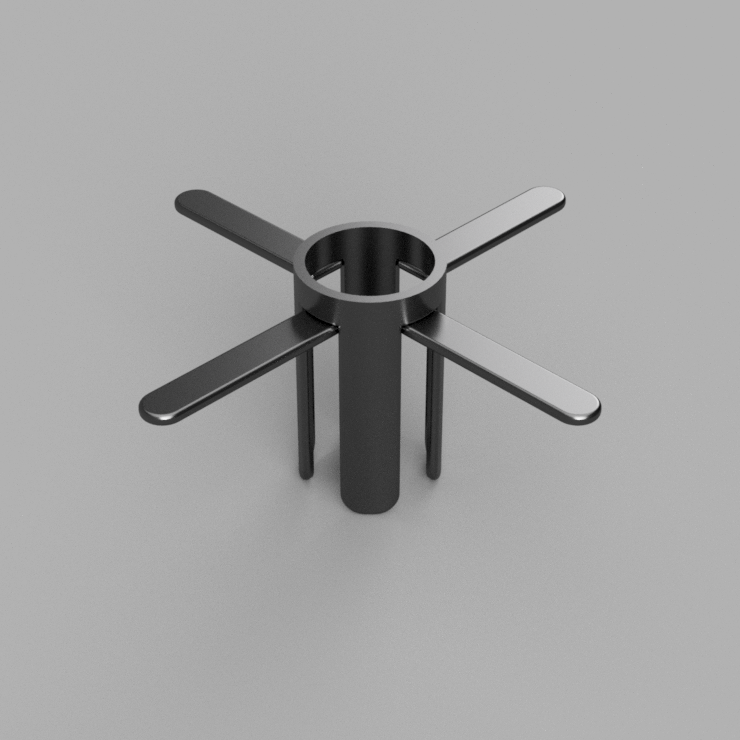
\includegraphics[width=0.6\textwidth]{resources/arm-folding-design.PNG}
    \caption{Arm Folding Design for CanSat: A compact folding mechanism that deploys after launch to optimize sensor exposure and maintain structural integrity.}
\end{figure}
\textbf{Description of Components:}
\begin{itemize}
    \item \textbf{Folding Arms}: Extend the motor arms to convert the CanSat into a drone configuration for controlled descent and hovering capabilities.
    \item \textbf{Hinge and Locking Mechanism}: Enables controlled deployment and secure retraction of the arms, ensuring stability under aerodynamic stresses.
    \item \textbf{Structural Frame}: Provides overall support and durability to the CanSat using lightweight yet robust materials.
\end{itemize}
\textbf{Additional Mechanical Components:}
\begin{itemize}
    \item \textbf{Motors and Propellers}: Provide necessary thrust and maneuverability during flight.
    \item \textbf{Electronic Speed Controllers (ESCs)}: Regulate motor speeds to ensure efficient power delivery.
    \item \textbf{Flight Controller}: Acts as the central processing unit to integrate sensor data and maintain stable flight.
    \item \textbf{Servos}: Used to deploy the arms and release the parachute.
    \item \textbf{Batteries}: Supply power to all electrical components.
\end{itemize}

\subsection{Electrical Design}
Below is an example power budget and component list based on typical values for cross-compatible components:
\begin{table}[H]
\centering
\begin{tabular}{|l|c|c|c|}
\hline
\textbf{Device} & \textbf{Voltage (V)} & \textbf{Current (mA)} & \textbf{Power (mW)} \\ \hline
RP2040 (Pi Pico Board) & 5 & 100 & 500 \\ \hline
RP2040 (Standalone Board) & 5 & 100 & 500 \\ \hline
Display Module & 5 & 20 & 100 \\ \hline
Buzzer & 5 & 20 & 100 \\ \hline
3 LEDs & 5 & 60 & 300 \\ \hline
Flight Controller (FC) & 5 & 150 & 750 \\ \hline
4 ESCs (idle) & 5 & 80 & 400 \\ \hline
Radio Receiver & 5 & 30 & 150 \\ \hline
4 Motors (average load) & 5 & 800 & 4000 \\ \hline
2 Servos & 5 & 300 & 1500 \\ \hline
Camera Module & 5 & 50 & 250 \\ \hline
\textbf{Total} & 5 & 1710 & 8550 \\ \hline
\end{tabular}
\caption{Example Power Budget and Component List}
\end{table}
Assuming a 5\,V system, the estimated current consumption is about 1710\,mA (approximately 8.55\,W). To achieve over 4 hours of operation, we propose a battery of at least 7500\,mAh. For example, a 7.4\,V LiPo battery paired with an efficient buck converter ($\approx$90\% efficiency) would yield roughly 4.4 hours of runtime under continuous load. These estimates assume typical operating conditions; duty cycles may reduce average consumption further.

\subsection{Radio Design}
For our CanSat project, we leverage the Challenger RP2040 LoRa module for robust, long-range communication with a dedicated ground station. This low-power, spread-spectrum module is ideal for compact unmanned systems. Key design options include:
\begin{itemize}
    \item \textbf{Frequency Band Selection:} Regionally compliant frequencies (e.g., 915 MHz in North America, 868 MHz in Europe) to optimize propagation and minimize interference.
    \item \textbf{Antenna Configuration:} A high-gain directional antenna at the ground station (with optional LNA) to extend range and improve signal quality.
    \item \textbf{Diversity Reception:} Multiple ground station antennas to mitigate multipath fading and improve reliability in dynamic conditions.
    \item \textbf{Software-Defined Radio (SDR):} Techniques to allow dynamic frequency adjustments and advanced signal processing for increased robustness.
\end{itemize}
These strategies, combined with the Challenger RP2040 LoRa module, ensure a resilient RF design for our CanSat system.

\subsection{Software Design}
Our software architecture comprises several modules. The primary module manages basic functionality: sensors record and store values on an SD card while periodically transmitting data via radio. The guided descent module uses onboard sensors—such as gyroscopes—to correct for wind disturbances. Additionally, camera inputs stabilize PID values to prevent overcorrection. This is achieved by integrating machine learning, specifically Convolutional Neural Networks (CNNs), to detect the horizon in real-time, evaluate its angle, and compute necessary corrections.

\subsection{Recovery System}
Our recovery system features a controlled descent mechanism that allows precise landing location and timing selection. The drone is designed to hover at approximately 20 meters, maintaining a stable altitude while automatically centring itself back to its launch point or a designated safe landing site.

\section{Project Planning}

\subsection{Time Schedule}
\begin{enumerate}
    \item \textbf{Concept Development \& Initial Planning (February – Early March 2025)}
    \begin{itemize}
        \item Define mission objectives and software architecture.
        \item Conduct feasibility studies and technical research.
        \item Begin drafting the Personal Preliminary Design Report (March 5th, 2025).
    \end{itemize}
    \item \textbf{Preliminary Design \& Outreach Preparation (Early – Mid March 2025)}
    \begin{itemize}
        \item Submit the Preliminary Design Report (March 9th, 2025).
        \item Conduct outreach sessions with junior classes (March 6th \& 13th, 2025).
        \item Initiate company outreach efforts (March 8th, 2025).
    \end{itemize}
    \item \textbf{Software Development \& Testing (Mid March – Early April 2025)}
    \begin{itemize}
        \item Implement core sensor data logging and transmission.
        \item Develop and test the guided descent module (including PID control and CNN-based horizon detection).
        \item Conduct simulations and refine machine learning models.
    \end{itemize}
    \item \textbf{System Integration \& Full Testing (April 2025)}
    \begin{itemize}
        \item Integrate and test all software modules.
        \item Conduct elementary school outreach (April 2025).
        \item Prepare for competition and finalize deployment procedures.
    \end{itemize}
    \item \textbf{CanSat Competition \& Launch (Late April 2025)}
    \begin{itemize}
        \item Participate in the CanSat Competition Weekend (April 24th, 2025).
        \item Execute the CanSat launch (April 26th, 2025).
        \item Analyze performance data and document results.
    \end{itemize}
\end{enumerate}

\subsection{Resource Estimation}

\subsubsection{Budget}
\begin{itemize}
    \item Mainboard: \$20
    \item Flight Controller: \$50
    \item Motors (x4): \$100
    \item Sensors (e.g., IMU, environmental sensors): \$30
    \item SD Card Module and Storage: \$10
    \item Radio Transceiver Module: \$20
    \item Battery Pack and Power Management: \$30
    \item Structural Materials and Enclosure: \$15
    \item Wiring, Connectors, and Miscellaneous Electronics: \$10
    \item Contingency and Additional Hardware: \$15
\end{itemize}

\subsubsection{External Support}
\begin{itemize}
    \item \textbf{Manufacturing Companies}
    \begin{itemize}
        \item \textbf{Packet Digital}: Specializes in power management and system integration for UAS, offering custom battery and charger designs.
        \item \textbf{Composites Technology Research Malaysia (CTRM)}: Produces UAVs like the Aludra and components for major aircraft manufacturers.
    \end{itemize}
    \item \textbf{Sponsorships}
    \begin{itemize}
        \item \textbf{National Science Foundation (NSF)}
        \item \textbf{Anduril Industries}: Secured a \$642 million contract with the U.S. Marine Corps.
    \end{itemize}
    \item \textbf{Subject Matter Experts (SMEs)}
    \begin{itemize}
        \item \textbf{Vic Moss}: Expert on U.S. drone regulation.
        \item \textbf{Brandon Karr}: Expert in UAS operations for public safety.
    \end{itemize}
    \item \textbf{Academic Institutions}
    \begin{itemize}
        \item \textbf{FAA Drone and Advanced Air Mobility (AAM) Symposium}
    \end{itemize}
    \item \textbf{Regulatory Agencies}
    \begin{itemize}
        \item \textbf{Federal Aviation Administration (FAA)}
    \end{itemize}
    \item \textbf{Community Engagement}
    \begin{itemize}
        \item \textbf{Police Executive Research Forum (PERF)}
    \end{itemize}
\end{itemize}

\subsection{Test Plan}
\begin{enumerate}
    \item \textbf{Individual System Testing}
    \begin{itemize}
        \item Calibrate and validate sensors (IMU, environmental).
        \item Test motors individually for responsiveness.
        \item Assess flight controller via bench tests and in-flight evaluations.
        \item Verify radio communication range and reliability.
        \item Evaluate battery performance under different loads.
        \item Conduct structural stress tests.
        \item Inspect wiring and connectors.
    \end{itemize}
    \item \textbf{Integrated System Testing}
    \begin{itemize}
        \item Perform test flights in windy conditions.
        \item Analyze CNN-based autonomous correction capabilities.
        \item Use simulators for various altitude scenarios.
    \end{itemize}
    \item \textbf{Compliance with Standards}
    \begin{itemize}
        \item \textbf{DO-160}: Verify environmental stress withstand.
        \item \textbf{DO-178C}: Ensure software meets safety and performance criteria.
        \item \textbf{FAA Order 8130.34}: Follow airworthiness certification procedures.
    \end{itemize}
\end{enumerate}

\section{Outreach Programme}
Our outreach programme engages youth in STEM through hands-on workshops and interactive activities focused on electronics and programming. In addition to in-person events, our Instagram page showcases our recent CanSat activities.
\begin{itemize}
    \item \textbf{Junior Outreach: Foundations Math 10, Fraser Heights Secondary}\\
    Presentation and Circuit Schematics Activity, March 6th, 2025.
    \item \textbf{Junior Outreach \#2: Drafting 9/10, Fraser Heights Secondary}\\
    Presentation and Microcontroller Workshop, March 13th, 2025.
    \item \textbf{Elementary Outreach: BASES, Erma Stephenson Elementary}\\
    Circuit and Breadboard Building Workshop (Date TBD).
    \item \textbf{Elementary Outreach \#2: Berkshire Park Elementary}\\
    Microcontroller and Beginner Level Coding Workshop (Date TBD).
    \item \textbf{Community Outreach: TBD}
\end{itemize}

\section{Requirements Verification}
\begin{table}[H]
\centering
\begin{tabular}{|l|l|}
\hline
\textbf{Parameter} & \textbf{Value} \\ \hline
Height of the CanSat & $<$115 mm \\ \hline
Mass of the CanSat & TBD \\ \hline
Diameter of the CanSat & $<$66 mm \\ \hline
Flight Time & TBD \\ \hline
Calculated Descent Rate & 7 m/s \\ \hline
Operational Duration (ON) & TBD \\ \hline
Total Cost & TBD \\ \hline
\end{tabular}
\caption{CanSat Requirements Verification Parameters}
\end{table}

\end{document}
